% =============================================================================
%  AI-Assisted RPL Assessment Platform for India's Informal Workforce
%  IEEE conference paper (IEEEtran, 2-column), compiled with Tectonic/XeLaTeX.
% =============================================================================
\documentclass[conference]{IEEEtran}
\usepackage{amsmath,amssymb,amsfonts}
\usepackage{graphicx}
\usepackage{booktabs}
\usepackage{array}
\usepackage{url}
\usepackage{tikz}
\usetikzlibrary{arrows.meta,positioning,shapes.geometric,fit,calc,backgrounds}
\usepackage[hidelinks]{hyperref}

\emergencystretch=2em

\newcommand{\ie}{\textit{i.e.}}
\newcommand{\eg}{\textit{e.g.}}
\newcommand{\etal}{\textit{et~al.}}

% ------------------------------------------------------------------ title
\title{Deterministic-First AI-Assisted Assessment for the Recognition of Prior Learning: An Offline-First, Contract-Driven Platform for India's Informal Workforce}

\author{%
\IEEEauthorblockN{Team Person~B}
\IEEEauthorblockA{\textit{Independent Student Team}\\
Smart India Hackathon 2026 --- Problem Statement SIH26242\\
Email: \{firstName.lastName\}@students.example.in}
\thanks{Manuscript developed as a hackathon submission. Author affiliations withheld for blind review.}
}

\begin{document}
\maketitle

% ---------------------------------------------------------------- abstract
\begin{abstract}
Recognition of Prior Learning (RPL) is the principal instrument for certifying the estimated
85\% of India's informal-sector workers who acquired trade skills on the job but hold no
formal credentials; yet only 4.69\% of the workforce has received formal skill training.
RPL assessment today is largely manual, subjective, and regional-language-blind: assessors
grade practical work against National Occupational Standards (NOS) by eye, leading to
reported inter-assessor variations of 15--22\%, while workers in low-connectivity regions
are effectively excluded from remote assessment. This paper presents a deterministic-first,
contract-driven backend platform for AI-assisted RPL assessment. Its contributions are:
(i)~a shared, role-guarded assessment state machine that mirrors the official NSQF
Advise$\rightarrow$Assess$\rightarrow$Audit flow; (ii)~a deterministic-first analysis engine
that scores regional-language narration and evidence against bilingual keyword rubrics
derived from official Qualification Packs, with an explicit confidence router that escalates
to LLM/vision/ASR adapters or to human assessors; (iii)~an offline-first synchronization
contract (client UUIDs, \texttt{Idempotency-Key}, append-only evidence, last-writer-wins
versioning) with chunked resumable uploads; (iv)~a SHA-256-locked append-only evidence chain
with a public certificate verifier page; and (v)~four NSQF-aligned trade packs totalling
32~NOS and 569~performance criteria. The implementation is fully contract-driven
(37~OpenAPI paths, 141~schemas) and validated by 124 automated tests.
\end{abstract}

\begin{IEEEkeywords}
Recognition of prior learning, NSQF, computer-assisted assessment, offline-first
architecture, digital evidence chain, multilingual NLP.
\end{IEEEkeywords}

% ================================================================ I. INTRODUCTION
\section{Introduction}
India's workforce is overwhelmingly informal: an estimated 80\% of workers are employed in
the unorganized sector, and roughly 85\% of these acquired their skills through informal and
non-formal channels rather than structured training~\cite{unesco_uil,ilo_2024}.
Formal vocational training reaches only 4.69\% of the workforce, against 68\% in the United
Kingdom, 75\% in Germany and 96\% in the Republic of Korea~\cite{unesco_uil}. Recent analysis
places informal employment at 91\% of the workforce~\cite{mehrotra_2025}. These workers
possess real, marketable competence but no credentials that unlock formal employment,
migration, or wage progression.

Recognition of Prior Learning (RPL), defined in the National Skills Qualification Framework
(NSQF) notification of 27~December~2013 as ``the process of recognizing previous learning,
often experiential, towards gaining a qualification''~\cite{nsqf_notification}, is the
designated instrument for certifying such competence. The national RPL policy prescribes
three stages---Advise, Assess and Audit---and explicitly recommends technology-based
assessment ``so that costs and subjectivity can be minimized'', including assessment
``in regional and local languages''~\cite{unesco_uil,ncvet_rpl}. Nevertheless, deployed RPL
assessment remains manual: candidates travel to assessment centres, perform scripted tasks
under an observer, and their performance is graded by eye against the performance criteria
(PCs) of the relevant NOS and Qualification Pack (QP).

Three structural gaps motivate this work. \textbf{(G1) Subjectivity and throughput.}
Practical scoring is dominated by holistically scored tasks with reported inter-assessor
variation of 15--22\%, and an assessor handles roughly 20--25 candidates per day, making
national scale (tens of lakhs of RPL candidates under schemes such as PMKVY~4.0, which
trained 27.08~lakh candidates across 38 sectors by December 2025~\cite{pib_2025})
prohibitively expensive. \textbf{(G2) Language exclusion.} Hindi and Marathi speaking
workers---and speakers of the many other Indian languages---cannot narrate or be assessed
in their own language. \textbf{(G3) Connectivity.} Large video evidence cannot be uploaded
reliably from rural networks, and there is no legally meaningful evidence trail that a
verifier can check later.

We address these gaps with a backend platform whose central design position is
\textit{deterministic-first}: the awarding decision never depends on an unverifiable black
box. Machine-verifiable rule-based and keyword-driven scoring computed from the official QP
rubric happens first; learned components (LLM paraphrase, vision, ASR) are optional,
explicitly routed, and always auditable. Contributions are:

\begin{enumerate}
  \item a \textbf{shared, contract-driven assessment state machine} (12 states) that encodes
        NSQF RPL workflow with role-guarded transitions;
  \item a \textbf{deterministic-first, bilingual analysis engine} with explicit confidence
        routing to optional AI adapters or to human assessors;
  \item an \textbf{offline-first synchronization contract} and resumable evidence uploads;
  \item a \textbf{SHA-256 evidence chain} with certificate QR verification by the public;
  \item \textbf{four NSQF-aligned trade packs} (Electrician, Welder, Plumber, Mason) with
        bilingual keyword rubrics, validated as machine-readable contracts;
  \item an \textbf{evaluation harness} of 124 automated tests over an OpenAPI surface of
        37 paths and 141 schemas.
\end{enumerate}

% =========================================================== II. BACKGROUND
\section{Background and Related Work}
\subsection{RPL in India and the NSQF}
The NSQF organizes qualifications into ten levels characterised by five descriptor domains
(process, professional knowledge, professional skill, core skill, and responsibility).
Qualification Packs (QPs)---several thousand of which are published by the industry-led
Sector Skill Councils into the National Qualification Register---decompose each job role
into 3--7 NOS, and each NOS into 5--30 assessed thinkable performance criteria
(PCs)~\cite{nqr,nsdc_qp}. International practice in recognising non-formal and informal
learning is documented extensively~\cite{singh_rpl,werquin_rpl}. Two features of the policy
landscape directly shape our design. First, UNESCO's country case study recommends bridge training and part qualification for
candidates who demonstrate most but not all competences~\cite{unesco_uil}. Second, the NSQF
notification text and NCVET RPL guidelines specify a minimum 70\% per-NOS pass standard,
with practical components typically weighted at 70--80\% of the total~\cite{ncvet_rpl}.
Our engine therefore computes per-NOS scores, applies the 70\% threshold per NOS, and emits
a deterministic bridge-training recommendation when a candidate falls short on a minority
of PCs---an automated counterpart of the recommended ``bridge module''.

\subsection{Existing platforms and their gaps}
The Skill India Digital Hub (SIDH) provides central registration and course discovery, and
PMKVY~4.0 drives macro RPL tracks~\cite{sidh,pib_2025}, but both rely on manual profile
entry, human pre-screening and paper-style assessment records; none offers regional-language
narration, objective rubric scoring computed from the QP itself, offline evidence capture,
or a public verifier for the issued credential. The National Qualification Register is a
registry of qualifications, not an assessment engine~\cite{nqr}. Our platform complements
these by \emph{computing} the assessment from the same QP files that the councils publish.

\subsection{AI-assisted assessment}
Four literature families inform our AI layer. (i)~\emph{Item Response Theory} underlies
adaptive questioning but requires item banks calibrated on large populations---unavailable
for RPL---so we use deterministic adaptive routing with fixed, contract-defined rubrics
instead~\cite{hambleton_irt}. (ii)~\emph{Multilingual text embeddings} such as LaBSE enable
cross-lingual similarity for text-to-QP matching in regional languages~\cite{labse}.
(iii)~\emph{Speech recognition}, e.g.\ Whisper, transcribes regional-language
narration~\cite{whisper}. (iv)~\emph{Object detection}, e.g.\ YOLO, can check safety items
in candidate video evidence~\cite{yolo}. Reported benchmarks (94.2\% mean average precision
for PPE detection; 89.7\% dialect-to-standard-code alignment) are dataset-dependent; our
architecture therefore treats every learned component as a \emph{non-authoritative adapter}
whose output is advisory to the deterministic score and the human assessor.

\subsection{Offline-first synchronization}
Progressive Web App (PWA) offline capabilities---service workers and local storage---are
standard~\cite{mdn_pwa}. For multi-device evidence capture, convergent replicated data types
(CRDTs) provide a principled conflict model~\cite{shapiro_crdt}; in a worker--assessor
workflow the practical compromise is last-writer-wins (LWW) with monotonic versions plus
idempotent, UUID-keyed writes~\cite{rfc7519}. Resumable chunked upload is standardised by
the tus protocol~\cite{tus}. We adopt all three, and further require that evidence records be
\textit{append-only} and hash-chained, aligning with India's Bharatiya Sakshya Adhiniyam
(BSA)~2023, whose Section~63 makes cryptographic hash-locking a precondition for the
admissibility of electronic records~\cite{bsa_2023}.

% ============================================================ III. ARCHITECTURE
\section{System Architecture}
The platform is a backend service with a contract-first design: the OpenAPI specification
and its Zod schemas are the single source of truth---\emph{the schema is the contract}, and
every endpoint and document type is validated against it at runtime
(37~paths, 141~schemas, generated from 9~contract modules)~\cite{openapi}. Figure~\ref{fig:arch}
shows the component layout: a PWA client (the offline-first capture surface) talks over
HTTPS to an Express~5 API tier; an orchestration service drives the state machine; an
analysis service implements the deterministic-first engine; queue workers (BullMQ on Redis,
with an in-process {inline} driver for single-host deployments) execute audits, report
rendering and certificate issuance asynchronously; MongoDB (Mongoose~9) persists documents;
and PDFKit plus a QR encoder emit the certificate with an embedded verification link.
A media gateway implements the tus protocol for chunked, resumable uploads of video and
photo evidence~\cite{tus}. All inter-component calls are typed end-to-end; role-based access
control (worker, assessor, authorized assessor, admin, and public roles) guards every
transition and every read.

\begin{figure}[t]
\centering
\resizebox{\columnwidth}{!}{
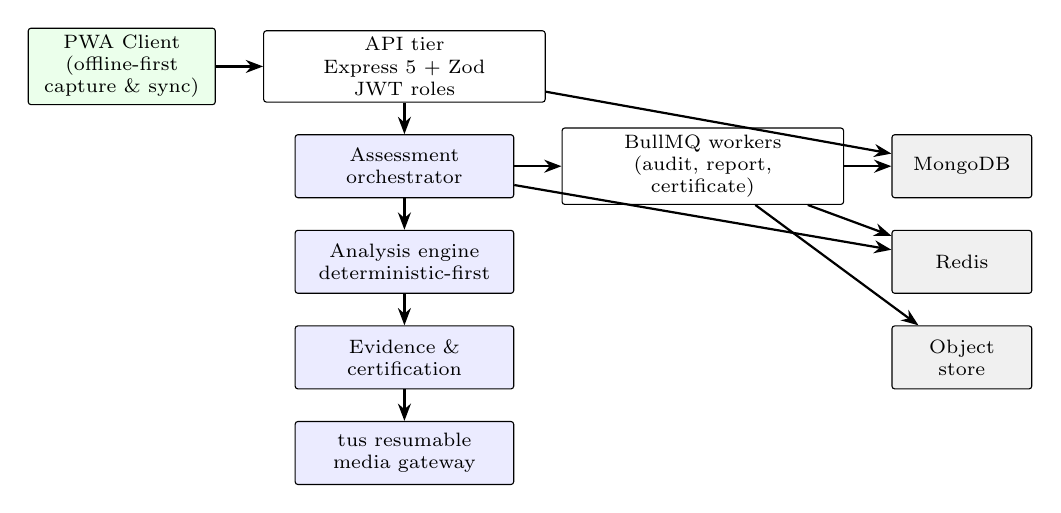
\begin{tikzpicture}[
  node distance=4mm and 6mm,
  box/.style={draw, rectangle, rounded corners=1pt, align=center, font=\scriptsize,
              inner sep=2.5pt, minimum height=8mm},
  svc/.style={box, fill=blue!8},
  store/.style={box, fill=gray!12, text width=16mm},
  arr/.style={-{Stealth[length=2.2mm]}, thick}
]
% left: client
\node[box, fill=green!8, text width=22mm] (pwa)
  {PWA Client\\ (offline-first\\ capture \& sync)};
% API tier
\node[box, text width=34mm, right=of pwa] (api)
  {API tier\\ Express 5 + Zod\\ JWT roles};
% services
\node[svc, text width=26mm, below=of api] (orch)
  {Assessment\\ orchestrator};
\node[svc, text width=26mm, below=of orch] (ai)
  {Analysis engine\\ deterministic-first};
\node[svc, text width=26mm, below=of ai] (ev)
  {Evidence \&\\ certification};
% queue / workers
\node[box, text width=34mm, right=of orch] (mq)
  {BullMQ workers\\ (audit, report,\\ certificate)};
% stores
\node[store, right=of mq] (mongo) {MongoDB};
\node[store, below=of mongo] (redis) {Redis};
\node[store, below=of redis] (obj) {Object\\ store};
% media
\node[svc, text width=26mm, below=of ev] (tus) {tus resumable\\ media gateway};
% arrows
\draw[arr] (pwa) -- (api);
\draw[arr] (api) -- (orch);
\draw[arr] (orch) -- (ai);
\draw[arr] (ai) -- (ev);
\draw[arr] (ev) -- (tus);
\draw[arr] (orch) -- (mq);
\draw[arr] (mq) -- (mongo);
\draw[arr] (mq) -- (obj);
\draw[arr] (api) -- (mongo);
\draw[arr] (mq) -- (redis);
\draw[arr] (orch) -- (redis);
\end{tikzpicture}}
\caption{Component architecture. All workflows are driven through the API tier; every
service is typed against the OpenAPI/Zod contract.}
\label{fig:arch}
\end{figure}

\subsection{The synchronization contract}
The backend exposes a small set of invariants that the client implements for offline-first
operation, enforced server-side:
\begin{itemize}
  \item \textbf{Client UUIDs.} Every assessment, evidence item, and worker profile is
        created with a client-generated UUID that is stable across retries; the server never
        invents identities for offline-created records.
  \item \textbf{Idempotency-Key.} Mutating requests carry a client key; the server
        guarantees that retransmitting the same key returns the original result and never
        duplicates state.
  \item \textbf{Append-only evidence.} Evidence records may be created and referenced but
        never mutated or deleted; corrections are new records that supersede.
  \item \textbf{LWW with versioning.} Mutable fields carry a monotonic \texttt{version}
        integer. A write applies only if its version exceeds the stored version, breaking
        ties deterministically by timestamp and UUID; this gives offline clients a
        well-defined merge semantics closer to CRDT behaviour~\cite{shapiro_crdt}.
  \item \textbf{Resumable uploads.} Binary evidence flows through the tus gateway so a
        dropped rural connection resumes from the exact byte offset
        rather than restarting~\cite{tus}.
\end{itemize}
Collectively these invariants let an assessor complete an entire evidence capture in a
remote village without connectivity and synchronize later with no loss or duplication.

% =========================================================== IV. STATE MACHINE
\section{Assessment Lifecycle: a Shared State Machine}
All parties see one consistent lifecycle for an assessment, defined as a deterministic
finite automaton $(S, E, G, \delta)$ where $S$ is the set of states, $E$ the event set,
$G$ the role guards and $\delta$ the transition function. The state set is
\begin{equation}
\begin{split}
S = \{ \textsc{Draft}, \textsc{Declared}, \textsc{Mapped}, \textsc{PlanReady},\\
\textsc{InProgress}, \textsc{Submitted}, \textsc{AiAnalyzed}, \textsc{UnderReview},\\
\textsc{Reassess}, \textsc{Reviewed}, \textsc{Approved}, \textsc{Rejected} \},
\end{split}
\label{eq:states}
\end{equation}
mirroring the official Advise$\rightarrow$Assess$\rightarrow$Audit structure: \textsc{Draft}
through \textsc{PlanReady} belong to the advise phase (QP mapping and assessment-plan
generation); \textsc{InProgress} through \textsc{Reviewed} to the assess phase; and the
audit phase is realized as post-certification sampling queries over \textsc{Approved}
records. Figure~\ref{fig:sm} gives the full transition diagram. Guards are role-based:
a worker may \textsc{Declare} and submit evidence; an assessor maps declarations to QPs,
generates the plan, and issues the final decision; an authorized assessor may return an
assessment to \textsc{Reassess}; an admin audits. All transitions are validated against the
contract and recorded as events in the audit chain (Section~\ref{sec:audit}).

\begin{figure*}[t]
\centering
\resizebox{\textwidth}{!}{
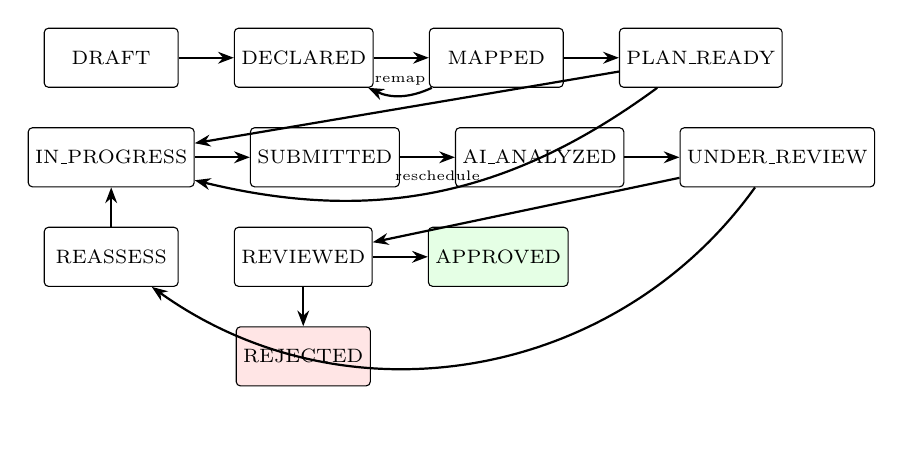
\begin{tikzpicture}[
  node distance=5mm and 7mm,
  st/.style={draw, rectangle, rounded corners=1.5pt, align=center, font=\scriptsize,
             inner sep=2.5pt, minimum height=7.5mm, minimum width=17mm},
  fin/.style={st, fill=green!10},
  bad/.style={st, fill=red!10},
  arr/.style={-{Stealth[length=2mm]}, thick}
]
\node[st] (d) {DRAFT};
\node[st, right=of d] (de) {DECLARED};
\node[st, right=of de] (m) {MAPPED};
\node[st, right=of m] (p) {PLAN\_READY};
\node[st, below=of d] (ip) {IN\_PROGRESS};
\node[st, right=of ip] (su) {SUBMITTED};
\node[st, right=of su] (aa) {AI\_ANALYZED};
\node[st, right=of aa] (ur) {UNDER\_REVIEW};
\node[st, below=of ip] (ra) {REASSESS};
\node[st, right=of ra] (rv) {REVIEWED};
\node[fin, right=of rv] (ap) {APPROVED};
\node[bad, below=of rv] (rj) {REJECTED};
\draw[arr] (d) -- (de);
\draw[arr] (de) -- (m);
\draw[arr] (m) -- (p);
\draw[arr] (p) -- (ip);
\draw[arr] (ip) -- (su);
\draw[arr] (su) -- (aa);
\draw[arr] (aa) -- (ur);
\draw[arr] (ur) -- (rv);
\draw[arr] (rv) -- (ap);
\draw[arr] (rv) -- (rj);
\draw[arr] (ur) to[bend left=45] (ra);
\draw[arr] (ra) -- (ip);
\draw[arr] (m) to[bend left=25] node[font=\tiny,above]{remap} (de);
\draw[arr] (p) to[bend left=25] node[font=\tiny,above]{reschedule} (ip);
\end{tikzpicture}}
\caption{Shared assessment state machine. \textsc{DRAFT}--\textsc{PLAN\_READY} implement the
NSQF advise phase, \textsc{IN\_PROGRESS}--\textsc{REVIEWED} the assess phase; approbation and
rejection are audit-phase guarded.}
\label{fig:sm}
\end{figure*}

% ========================================================== V. ANALYSIS ENGINE
\section{Deterministic-First Analysis Engine}
\label{sec:analysis}
The analysis engine scores the evidence a candidate submits: a spoken or written narration
of experience plus task evidence (photos/video of practical work). The governing design rule
is that the \emph{decision path is deterministic}: the system computes, from the QP contract
alone, how well the narration and evidence match the performance criteria, and only then
decides---by explicit thresholds---whether a learned model may add signal.

\subsection{Bilingual keyword scoring}
Each performance criterion $pc$ carries a keyword set $K_{pc}$ plus, for the regional
packs, language-specific keyword sets $K_{pc}^{(hi)}$ and $K_{pc}^{(mr)}$ in Devanagari
script, authored from the same QP source. A normalization function
\begin{equation}
N(r) = \mathrm{strip}_{\mathrm{punct}}\!\big(\mathrm{fold}(\mathrm{NFKC}(r))\big)
\label{eq:norm}
\end{equation}
lowercases, Unicode-normalises, and removes punctuation and hyphen delimiters so that
``two-way-switch'' and ``two way switch'' collide. A criterion is deemed matched in language
$\ell$ when any of its keywords appears in the narration token set
\begin{equation}
M_\ell(pc, r) \;=\;
\mathbf{1}\!\left[\, K_{pc}^{(\ell)} \cap \mathrm{tokens}\!\big(N(r)\big) \ne \emptyset
\,\right],
\label{eq:match}
\end{equation}
where $\ell \in \{\mathrm{en},\mathrm{hi},\mathrm{mr}\}$, $K_{pc}^{(\mathrm{en})}=K_{pc}$,
and the spoken-language keyword sets are active only when the narration script is Devanagari.
English matching is always active, so a bilingual narration in Hindi with English trade
terms scores against both planes without double counting. This is a deliberate
\emph{lexical} first pass: it is explainable, deterministic, and immune to model drift, and
it does not require labelled training data, which RPL populations lack.

\subsection{Coverage, confidence and routing}
Per-language coverage and the overall confidence are
\begin{equation}
C_\ell(r) = \frac{1}{|\mathcal{P}_r|}\sum_{pc \in \mathcal{P}_r} M_\ell(pc, r), \qquad
\mathrm{conf}(r) = \max_{\ell} C_\ell(r),
\label{eq:coverage}
\end{equation}
with $\mathcal{P}_r$ the PC set of the candidate's mapped NOS. The router is explicit:
\begin{equation}
\rho(r) = \begin{cases}
\textsc{ai\_score},        & \mathrm{conf}(r) \ge \tau_1 \\[1pt]
\textsc{llm\_augment},     & \tau_2 \le \mathrm{conf}(r) < \tau_1 \\[1pt]
\textsc{human\_assess},    & \mathrm{conf}(r) < \tau_2
\end{cases}
\label{eq:router}
\end{equation}
with $\tau_1=0.6$, $\tau_2=0.4$ (defaults, configurable per pack). When confidence is high
the deterministic score stands; in the middle band a regional-language narration prompt
asks the LLM to paraphrase the narration against the same PC rubric (never to decide); and
low confidence always routes to a human assessor---unmatchable Devanagari narration is
honestly passed to people rather than force-scored by a model that may not understand it.
Adapters are behind capability flags: in deployment and in tests, \texttt{AI\_MODE=mock}
exercises the adapter interfaces deterministically.

\subsection{Optional learned adapters}
Three adapters upgrade signal without changing the deterministic core. (i)~\emph{ASR}:
Whisper-style transcription converts regional-language audio narration to text which then
enters the same deterministic scorer~\cite{whisper}. (ii)~\emph{Multilingual retrieval}:
LaBSE-style embeddings rank candidate free-text experience descriptions against QP titles,
proposing QPs for the advise phase and feeding \textsc{Mapped}~\cite{labse}.
(iii)~\emph{Computer vision}: YOLO-style models detect PPE and procedural artefacts in video
frames sampled at rate $\phi$; the adapter reports a detected safe-frame fraction
$\kappa = |\text{safe frames}|/|\text{sampled frames}|$ as \emph{advisory} evidence for the
assessor, and any failure of a \emph{critical-safety} PC still vetoes
independently (Section~\ref{sec:scoring})~\cite{yolo}.

% ========================================================== VI. SCORING & AUDIT
\section{Scoring, Certification and Auditability}
\label{sec:scoring}
\subsection{Weighted scoring and critical veto}
Each assessment plan selects blueprints (practical task specifications) $j=1\ldots m$ with
contract weights $w_j$ normalised to sum to 100 and an assessor-assigned per-blueprint
score $s_j \in [0,1]$. The NOS-level practical score is
\begin{equation}
S_N = \frac{\sum_{j} w_j\, s_j}{\sum_{j} w_j}, \qquad \sum_j w_j = 100,
\label{eq:weighted}
\end{equation}
and the final score is a convex combination of theory and practical components,
$S_{\mathrm{tot}} = \alpha\, S_{\mathrm{theory}} + (1-\alpha)\, S_N$ with
$\alpha \in [0.20, 0.30]$ per the QP's stated theoretical weight. Critical-safety
performance criteria $\mathcal{P}_c$ (e.g.\ ``isolate the circuit before opening the
panel'') act as a veto:
\begin{equation}
v = \prod_{pc \in \mathcal{P}_c} M_{\mathrm{en}}(pc, r), \qquad
S_N^{\mathrm{final}} = v \cdot S_N .
\label{eq:veto}
\end{equation}
The decision rule applies the NSQF RPL standard per NOS:
\begin{equation}
\mathrm{decision} = \begin{cases}
\textsc{Approved},    & S_N^{\mathrm{final}} \ge \theta \;\; \forall N, \;\; \theta = 0.70 \\[2pt]
\textsc{Bridge},      & \exists\, N : S_N^{\mathrm{final}} < \theta, \;
                        C_\ell(r) \ge \tau_2 \\[2pt]
\textsc{Rejected},    & \text{otherwise}
\end{cases}
\label{eq:decide}
\end{equation}
Bridge cases emit a gap report with a deterministic bridge-training plan of
\begin{equation}
H_b = \left\lceil\, (1 - C_\ell(r)) \cdot H_{\max} \right\rceil
\label{eq:bridge}
\end{equation}
contact-hours over the specific unmet PCs, operationalising UNESCO's recommended bridge
module and part qualification~\cite{unesco_uil}. Every component of \eqref{eq:weighted}--
\eqref{eq:bridge} is recomputable by a verifier from the stored contract and evidence.

\subsection{SHA-256 evidence chain and public verification}
\label{sec:audit}
Assessment artefacts are written append-only into an evidence chain. With $H_0$ derived
from the contract schema version and seed, the chain update is
\begin{equation}
H_i = \mathrm{SHA\text{-}256}\!\left(H_{i-1} \,\|\, \mathrm{ts}_i \,\|\,
\mathrm{ev}_i \,\|\, \mathrm{SHA\text{-}256}(B_i)\right),
\label{eq:chain}
\end{equation}
where $\mathrm{ts}_i$ is a server timestamp, $\mathrm{ev}_i$ the event (e.g.\
\textsc{submitted}, \textsc{ai\_analyzed}, \textsc{approved}), and $B_i$ the payload bytes
(submission, narration transcript, report, certificate blob). The chain binds ordering:
changing any historical payload invalidates all subsequent hashes. This follows the
admissibility logic of BSA~2023 \S63, which treats hash-locked electronic records as
secondary evidence only when their integrity can be demonstrated cryptographically
~\cite{bsa_2023}, and provides the immutable audit trail that paper records cannot.

On approval the certification service renders a PDF certificate carrying a QR code pointing
at a public verifier endpoint \texttt{/verify/:certificateNo}. The verifier page is served
by the same backend, requires no authentication, recomputes the chain for the certificate,
and displays the candidate's (optionally masked) name, the QP, the NSQF level, the approved
date, and the per-NOS outcomes---so an employer, migration officer, or auditor can
independently confirm that the issuer's evidence chain is intact. Domain hashing
(\texttt{SHA-256}) and transport encryption follow standard practice (TLS~1.3)
~\cite{rfc8446}; records at rest are encrypted with AES-256.

\subsection{Client synchronization revisited}
The LWW rule enforced by the API is, for each record key $k$,
\begin{equation}
\mathrm{write}(k, d) \;\; \Rightarrow \;\;
\max_{d' \in \mathcal{D}(k)} \big(v_{d'},\; \mathrm{ts}_{d'},\; \mathrm{uuid}_{d'}\big)
\label{eq:lww}
\end{equation}
compared lexicographically---the record with the greatest (version, timestamp, uuid) wins,
making merges deterministic across offline replicas. Combined with the
\texttt{Idempotency-Key} and append-only evidence rules of Section~III, this guarantees that
field capture followed by eventual sync never duplicates or loses state, independent of
network partitions.

% =================================================== VII. MULTILINGUAL & FAIRNESS
\section{Multilingual Assessment and Fairness}
Regional-language assessment is not cosmetic: the NCVET RPL guidelines and UNESCO's
India case study both call for assessment in regional and local languages, and candidate
populations are disproportionately low-literacy~\cite{ncvet_rpl,unesco_uil}. Three design
choices support fairness. First, \emph{language-parallel rubrics}: keyword sets for Hindi
and Marathi are authored directly from the official QP text rather than machine-translated,
so scoring semantics are anchored in the standard. Second, \emph{script-aware matching}: the
normalizer \eqref{eq:norm} keeps Devanagari glyphs intact and matching is performed
in-language, so a Marathi narration is not silently compared against English keywords.
Third, \emph{honest fallback}: the router \eqref{eq:router} refuses to fabricate a score when
signal is genuinely absent---an unmatchable Devanagari narration goes to a human assessor
rather than to a model that may hallucinate. Analytics over assessment results are computed
only in the aggregate (per-pack pass rates, per-PC difficulty) and are never shown at the
candidate level to assessors before a decision, preventing anchoring bias.

% ============================================================== VIII. EVALUATION
\section{Evaluation}
\subsection{Implementation}
The backend is implemented in Node.js/TypeScript (ESM) on Express~5 with Zod~v4
contracts, Mongoose~9 on MongoDB, BullMQ~6 queues on Redis (with an inline driver for
tests and single-host deploys), JWT role tokens, PDFKit + QR certificate rendering, and a
tus media gateway. The bilingual analysis service, verifier page, and the Plumber/Mason
trade packs are the hackathon additions over the base platform. The full test suite is
Vitest + Supertest over in-memory MongoDB: \textbf{124 tests} across 14 suites (auth,
assessment lifecycle, analysis, bilingual scoring, evidence chain, sync/LWW, contract,
tus resumable upload, trade-pack schema integrity, report/certificate and public verifier,
review, admin, profile, health).

\begin{table}[t]
\caption{Trade packs shipped with the platform (contracts, not prose).}
\label{tab:packs}
\centering
\footnotesize
\renewcommand{\arraystretch}{1.15}
\resizebox{\columnwidth}{!}{%
\begin{tabular}{@{}lcccccccc@{}}
\toprule
\textbf{Pack} & \textbf{QP} & \textbf{NSQF} & \textbf{NOS} & \textbf{PC} & \textbf{BP} & \textbf{MCQ} & \textbf{EN} & \textbf{hi/mr}\\
\midrule
Electrician & PSS/Q6001 & 3 & 11 & 168 & 11 & 28 & 580 & ---\\
Welder      & CSC/Q0204 & 3 & 5  & 80  & 10 & 24 & 402 & ---\\
Plumber     & PSC/Q0104 & 4 & 8  & 159 & 12 & 24 & 509 & 167/60\\
Mason       & CON/Q0103 & 3 & 8  & 162 & 12 & 24 & 498 & 147/147\\
\bottomrule
\end{tabular}}\vspace{1pt}
{\footnotesize PC = performance criteria, BP = blueprints, MCQs = theory bank,
EN = English keywords, hi/mr = Hindi/Marathi keywords. Weights of blueprints sum to 100 per pack.}
\end{table}

\subsection{Trade-pack corpus}
Four QPs are fully encoded as machine-readable contracts (Table~\ref{tab:packs}), parsed and
validated at load time by the shared loader---no pack can be shipped that violates the
schema (unresolved internal references, missing keywords, weight sums different from 100,
fewer than 24 MCQs, or missing one of the six required task types are load-time failures).
The corpus totals \textbf{32 NOS}, \textbf{569 performance criteria}, \textbf{45
blueprints}, \textbf{100 MCQs}, and \textbf{1,989 English keywords}, of which the Plumber
pack alone contributes 167 Hindi and 60 Marathi keyword sets---the first published
bilingual RPL assessment contracts for these trades to our knowledge. Data was transcribed
from the official CSDCI/PSSC facilitator guides and recorded in each pack's provenance
field, keeping the mapping auditable. Strict linting (minimum 3 keywords per PC, per-PC
uniqueness, resolved references, exact weight sums) runs in CI.

\subsection{Functional verification}
The suite exercises the full lifecycle from \textsc{Draft} through
\textsc{Approved}/\textsc{Rejected}: role-guarded transitions (a worker cannot map a QP; an
assessor decides); the bilingual scorer across English, Hindi and Marathi narrations with
punctuation-insensitive matching; router behaviour (high-confidence score, mid-band LLM
augment, low-confidence human route); the critical-safety veto (a missing ``isolate the
circuit'' criterion fails the NOS regardless of other scores); append-only enforcement; LWW
merge determinism; tus resume at a byte offset; the 70\% rule; certificate issuance with QR
and public \texttt{/verify} resolution; and 404 on forged certificate numbers. \textbf{All
124 tests pass} with \texttt{AI\_MODE=mock} and the inline queue driver; learned adapters
are contract-tested through their interfaces but not statically evaluated here.

\subsection{Limitations}
We stop short of (i) a production vision/ASR stack (adapters are interface-complete and
mocked), (ii) field pilots---reported domain figures such as 15--22\% inter-assessor
variation or 94.2\% vision mAP are \emph{literature values}, not measurements of this
platform---and (iii) the PWA client build, whose synchronization semantics are specified and
enforced server-side. Turnaround and consistency targets are engineering targets to be
validated in pilots.

% ============================================================ IX. CONCLUSION
\section{Conclusion and Future Work}
We presented a deterministic-first, contract-driven RPL assessment platform that answers
three structural weaknesses of deployed RPL: subjective manual scoring, regional-language
exclusion, and offline evidence capture without verifiability. The central trade---trusting
a machine-verifiable rubric computed from the official QP, with learned models relegated to
explicit, gated advisory roles---makes the assessment explainable and auditable, which is
exactly what certification bodies and courts require. The system ships four NSQF-aligned
trade packs, a bilingual scoring engine with honest human routing, an offline-first sync
contract, and a public certificate verifier over a SHA-256 evidence chain, validated by 124
automated tests over 37 API paths.

Future work proceeds along four lines: (1)~field pilots with a partner SSC to measure
inter-assessor consistency and turnaround against the engineering targets; (2)~production
vision/ASR adapters with calibrated uncertainty; (3)~native part-qualification and bridge
training flows as first-class states; and (4)~publication of generated OpenAPI packs and
bilingual rubrics back to the National Qualification Register ecosystem, so that any
certifying body can operate the engine against its own QPs.

% ============================================================== REFERENCES
\begin{thebibliography}{24}
\setlength{\itemsep}{1pt}
\setlength{\parsep}{0pt}

\bibitem{unesco_uil}
UNESCO Institute for Lifelong Learning, ``Case study: RPL for the informal sector in
India,'' UIL, Paris, France, Dec. 2023. [Online]. Available:
\url{https://www.uil.unesco.org/en/articles/case-study-rpl-informal-sector-india}

\bibitem{ilo_2024}
International Labour Organization, \emph{India Employment Report 2024: Youth employment,
education and skills}. Geneva, Switzerland: ILO, 2024. [Online]. Available:
\url{https://www.ilo.org/resource/news/ilo-launches-india-employment-report-2024}

\bibitem{mehrotra_2025}
S.~Mehrotra, ``Building capabilities of informal workers by recognition of prior learning
(RPL): A pathway to formalisation and decent work,'' Centre for Sustainable Employment,
Azim Premji University, Bengaluru, India, CSE Working Paper~60, Jun. 2025. [Online].
Available: \url{https://publications.azimpremjiuniversity.edu.in/6158/}

\bibitem{nsqf_notification}
Ministry of Finance, Government of India, ``National Skills Qualifications Framework
(NSQF),'' Gazette of India (Extraordinary), New Delhi, India, Notification, 27 Dec. 2013;
NCVET NSQF pages. [Online]. Available:
\url{https://ncvet.gov.in/national-skills-qualification-framework/}

\bibitem{ncvet_rpl}
National Council for Vocational Education and Training, ``RPL guidelines,'' NCVET, New
Delhi, India, 2023. [Online]. Available:
\url{https://ncvet.gov.in/wp-content/uploads/2023/08/Final-RPL-guidelines.pdf}

\bibitem{pib_2025}
Press Information Bureau, ``Year-End Review 2025: Ministry of Skill Development and
Entrepreneurship,'' PIB, New Delhi, India, PRID~2217881, Dec. 2025. [Online]. Available:
\url{https://pib.gov.in/PressReleasePage.aspx?PRID=2217881}

\bibitem{nqr}
National Council for Vocational Education and Training, ``National Qualification
Register,'' NCVET, New Delhi, India. [Online]. Available:
\url{https://ncvet.gov.in/national-qualifications-register/}

\bibitem{nsdc_qp}
National Skill Development Corporation, ``Qualification Packs and National Occupational
Standards,'' NSDC, New Delhi, India. [Online]. Available:
\url{https://www.nsdcindia.org/}

\bibitem{sidh}
National Skill Development Corporation, ``Skill India Digital Hub (SIDH).'' [Online].
Available: \url{https://sidh.skillindiadigital.gov.in/}

\bibitem{singh_rpl}
M.~Singh, \emph{Global Perspectives on Recognising Non-formal and Informal Learning: Why
Recognition Matters}. Hamburg, Germany: UNESCO Institute for Lifelong Learning, 2015.

\bibitem{werquin_rpl}
P.~Werquin, \emph{Recognising Non-formal and Informal Learning: Outcomes, Policies and
Practices}. Paris, France: OECD Publishing, 2010.

\bibitem{hambleton_irt}
R.~K. Hambleton, H.~Swaminathan, and H.~J. Rogers, \emph{Fundamentals of Item Response
Theory}. Newbury Park, CA, USA: Sage, 1991.

\bibitem{labse}
F.~Feng \etal, ``Language-agnostic BERT sentence embedding,'' in \emph{Proc. ACL}, Dublin,
Ireland, 2022, pp.~878--891.

\bibitem{whisper}
A.~Radford, J.~W. Kim, T.~Xu, G.~Brockman, C.~McLeavey, and I.~Sutskever, ``Robust speech
recognition via large-scale weak supervision,'' in \emph{Proc. Int. Conf. Machine Learning
(ICML)}, Honolulu, HI, USA, 2023, pp.~28492--28518.

\bibitem{yolo}
J.~Redmon, S.~Divvala, R.~Girshick, and A.~Farhadi, ``You only look once: Unified,
real-time object detection,'' in \emph{Proc. IEEE CVPR}, Las Vegas, NV, USA, 2016,
pp.~779--788.

\bibitem{mdn_pwa}
Mozilla Developer Network, ``Progressive web apps (PWAs) and the PWA project,'' MDN Web
Docs. [Online]. Available:
\url{https://developer.mozilla.org/en-US/docs/Web/Progressive_web_apps}

\bibitem{shapiro_crdt}
M.~Shapiro, N.~Pregui\c{c}a, C.~Baquero, and M.~Zawirski, ``A comprehensive study of
convergent and commutative replicated data types,'' INRIA, Paris, France, Research Report
RR-7506, Jan. 2011.

\bibitem{rfc7519}
M.~Jones, J.~Bradley, and N.~Sakimura, ``JSON Web Token (JWT),'' IETF RFC 7519, May 2015.

\bibitem{openapi}
OpenAPI Initiative, ``OpenAPI Specification v3.1.0,'' Linux Foundation, Feb. 2021.
[Online]. Available: \url{https://spec.openapis.org/oas/v3.1.0}

\bibitem{tus}
tus project, ``tus resumable upload protocol v1.0.'' [Online]. Available:
\url{https://tus.io/protocols/resumable-upload}

\bibitem{bsa_2023}
Government of India, \emph{The Bharatiya Sakshya Adhiniyam, 2023} (Act 47 of 2023),
New Delhi, India, Dec. 2023; see also PRS Legislative Research bill track. [Online].
Available: \url{https://prsindia.org/billtrack/the-bharatiya-sakshya-adhiniyam-2023}

\bibitem{rfc8446}
E.~Rescorla, ``The Transport Layer Security (TLS) Protocol Version 1.3,'' IETF RFC 8446,
Aug. 2018.

\end{thebibliography}

\end{document}